\documentclass[UTF8, 12pt]{ctexart}
% UTF8编码,ctexart现实中文
\usepackage{color}
% 使用颜色
\definecolor{orange}{RGB}{255,127,0}  
\definecolor{violet}{RGB}{192,0,255}  
\definecolor{aqua}{RGB}{0,255,255} 
\usepackage{geometry}
\setcounter{tocdepth}{4}
\setcounter{secnumdepth}{4}
% 设置四级目录与标题
\geometry{papersize={21cm,29.7cm}}
% 默认大小为A4
\geometry{left=3.18cm,right=3.18cm,top=2.54cm,bottom=2.54cm}
% 默认页边距为1英尺与1.25英尺
\usepackage{indentfirst}
\setlength{\parindent}{2.45em}
% 首行缩进2个中文字符
\usepackage{setspace}
\renewcommand{\baselinestretch}{1.5}
% 1.5倍行距
\usepackage{amssymb}
% 因为所以
\usepackage{amsmath}
% 数学公式
\usepackage[colorlinks,linkcolor=black,urlcolor=blue]{hyperref}
% 超链接
\usepackage{tikz}
% 绘图
\author{Didnelpsun}
\title{标题}
\date{}
\begin{document}
\maketitle
\pagestyle{empty}
\thispagestyle{empty}
\tableofcontents
\thispagestyle{empty}
\newpage
\pagestyle{plain}
\setcounter{page}{1}
\section{总体与样本}

\subsection{总体定义}

\textcolor{violet}{\textbf{定义:}}研究对象的全体称为\textbf{总体},组成总体的每一个元素称为\textbf{个体}。

\subsection{样本}

\subsubsection{定义}

\textcolor{violet}{\textbf{定义:}}$n$个相互独立且域总体$X$有相同概率分布的随机变量$X_1,X_2,\cdots,X_n$所组成的整体$(X_1,X_2,\cdots,X_n)$称为来自总体$X$,容量为$n$个一个\textbf{简单随机样本},简称\textbf{样本}。一次抽样结果的$n$个具体值$(x_1,x_2,\cdots,x_n)$称为来自样本$X_1,X_2,\cdots,X_n$的一个\textbf{观测值}或\textbf{样本值}。

在概率论中称为独立同分布,而在数理统计就称为简单随机样本。

\subsubsection{分布}

对于容量为$n$的样本$X_1,X_2,\cdots,X_n$有如下定理:假设总体$X$的分布函数为$F(x)$(概率密度为$f(x)$,或概率分布为$p_i=P\{X=x_i\}$),则$(X_1,X_2,\cdots,X_n)$的分布函数为$F(x_1,x_2,\cdots,x_n)=\prod\limits_{i=1}^nF(x_i)$。

对于离散型随机变量联合分布:$F(X_1=x_1,X_2=x_2,\cdots,X_n=x_n)=\prod\limits_{i=1}^nP\{X_i=x_i\}$。

对于连续型随机变量联合概率密度:$f(x_1,x_2,\cdots,x_n)=\prod\limits_{i=1}^nf(x_i)$。

\section{统计量与分布}

\subsection{统计量}

设$X_1,X_2,\cdots,X_n$来自总体$X$的一个样本,$g(x_1,x_2,\cdots,x_n)$为$n$元函数,若$g$中不含有任何未知参数,则称$g(X_1,X_2,\cdots,X_n)$为样本$X_1,X_2,\cdots,X_n$的一个\textbf{统计量}。若$(x_1,x_2,\cdots,x_n)$为样本值,则称$g(x_1,x_2,\cdots,x_n)$为$g(X_1,X_2,\cdots,X_n)$的\textbf{观测值}。

\subsection{常用统计量}

\begin{itemize}
    \item 样本均值:$\overline{X}=\dfrac{1}{n}\sum\limits_{i=1}^nX_i$。
    \item 样本方差:$S^2=\dfrac{1}{n-1}\sum\limits_{i=1}^n(X_i-\overline{X})^2$。
    \item 样本标准差:$S=\sqrt{\dfrac{1}{n-1}\sum\limits_{i=1}^n(X_i-\overline{X})^2}$。
    \item 样本$k$阶(原点)矩:$A_k=\dfrac{1}{n}\sum\limits_{i=1}^nX_i^k$($k=1,2,\cdots$)。
    \item 样本$k$中心矩:$B_k=\dfrac{1}{n}\sum\limits_{i=1}^n(X_i-\overline{X})^k$($k=1,2,\cdots$)。
\end{itemize}

\subsection{顺序统计量}

\subsubsection{概念}

将样本$X_1,X_2,\cdots,X_n$的$n$个观测量按其值从小到大的顺序排列,得到$X_{(1)}\leqslant X_{(2)}\leqslant\cdots\leqslant X_{(n)}$。

随机变量$X_{(k)}$($k=1,2,\cdots,n$)称为\textbf{第$k$顺序统计量},其中$X_{(1)}$是最小顺序统计量,而$X_{(n)}$是最大顺序统计量。

$X_{(n)}$的分布函数为$F_{(n)}(x)=[F(x)]^n$,概率密度为$f_{(n)}(x)=n[F(x)]^{n-1}f(x)$。

证明:$F_{(n)}(x)=P\{X_{(n)}\leqslant x\}=P\{\max\{x_1,\cdots,x_n\}\leqslant x\}=P\{x_1\leqslant x,\cdots,x_n\leqslant x\}=P\{x_1\leqslant x\}\cdots P\{x_n\leqslant x\}=F_{(1)}(x)\cdots F_{(n)}(x)=[F(x)]^n$。

$X_{(1)}$的分布函数为$F_{(1)}(x)=1-[1-F(x)]^n$,概率密度为$f_{(1)}(x)=n[1-F(x)]^{n-1}f(x)$。

证明:$F_{(1)}(x)=P\{X_{(1)}\leqslant x\}=P\{\min\{x_1,\cdots,x_n\}\leqslant x\}=1-P\{\min\{x_1,\cdots$\\$,x_n\}>x\}=1-P\{x_1>x,\cdots,x_n>x\}=1-P\{x_1>x\}\cdots P\{x_n>x\}=1-[1-P\{x_1\leqslant x\}]\cdots[1-P\{x_n\leqslant x\}]=1-[1-F_{(1)}(x)]\cdots[1-F_{(n)}(x)]=1-[1-F(x)]^n$。

\subsubsection{性质}

设总体$X$的期望$EX=\mu$,方差$DX=\delta^2$,样本$X_1,X_2,\cdots,X_n$取自$X$,$\overline{X}$和$S^2$分别为样本的均值和方差,则:

\begin{itemize}
    \item $EX_i=\mu$。
    \item $DX_i=\delta^2$。
    \item $E\overline{X}=EX=\mu$。
    \item $D\overline{X}=D\left(\dfrac{1}{n}\sum\limits_{i=1}^nx_i\right)=\dfrac{1}{n^2}n\delta^2=\dfrac{1}{n}DX=\dfrac{\delta^2}{n}$。
    \item $E(S^2)=E\left(\dfrac{1}{n-1}\sum\limits_{i=1}^n(x_i-\overline{x})^2\right)=E\left(\dfrac{1}{n-1}\sum\limits_{i=1}^n(x_i^2-2x_i\overline{x}+\overline{x}^2)\right)=$\\$E\left(\dfrac{1}{n-1}\left(\sum\limits_{i=1}^nx_i^2-2\overline{x}\cdot\sum\limits_{i=1}^nx_i+n\overline{x}^2\right)\right)=E\left(\dfrac{1}{n-1}\left(\sum\limits_{i=1}^nx_i^2-n\overline{x}^2\right)\right)=$\\$\dfrac{1}{n-1}E\left(\sum\limits_{i=1}^nx_i^2-n\overline{x}^2\right)=\dfrac{1}{n-1}\left(\sum\limits_{i=1}^nEx_i^2-nE\overline{x}^2\right)=\dfrac{n}{n-1}[(Ex_i)^2+Dx_i-(E\overline{x})^2-D\overline{x}]=\dfrac{n}{n-1}\left(\mu^2+\delta^2-\mu^2-\dfrac{\delta^2}{n}\right)=DX=\delta^2$。
\end{itemize}

\subsection{三大分布}

\subsubsection{\texorpdfstring{$\chi^2$分布}{}}

\paragraph{概念} \leavevmode \medskip

\textcolor{violet}{\textbf{定义:}}若随机变量$X_1,X_2,\cdots,X_n$相互独立,且都服从标准正态分布,则随机变量$X=\sum\limits_{i=1}^nX_i^2$服从自由度为$n$的$\chi^2$分布,记为$X\sim\chi^2(n)$,特别地$X_i^2\sim\chi^2(1)$。

对给定的$\alpha$($0<\alpha<1$)称满足$P\{\chi^2>\chi_\alpha^2(n)\}=\int_{\chi_\alpha^2(n)}^{+\infty}f(x)\,\textrm{d}x=\alpha$的$\chi_\alpha^2(n)$为$\chi^2(n)$分布的\textbf{上$\alpha$分位点}。

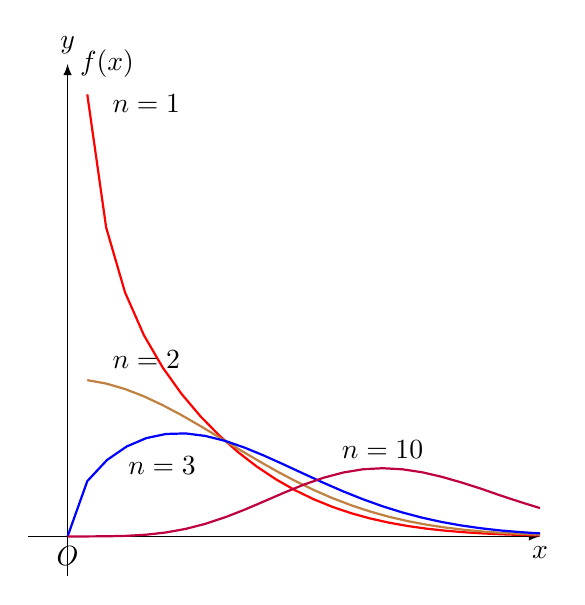
\begin{tikzpicture}[scale=2]
    \draw[-latex](-0.25,0) -- (3,0) node[below]{$x$};
    \draw[-latex](0,-0.25) -- (0,3) node[above]{$y$};
    \filldraw[black] (0,0) node[below]{$O$};
    \draw[red, thick, domain=0.125:3] plot (\x,{pow(\x,-0.5)*pow(e,-\x*\x/2)});
    \filldraw[black] (0.5,2.75) node{$n=1$};
    \draw[brown, thick, domain=0.125:3] plot (\x,{pow(e,-\x*\x/2)});
    \filldraw[black] (0.5,1.125) node{$n=2$};
    \draw[blue, thick, domain=0:3] plot (\x,{pow(\x,0.5)*pow(e,-\x*\x/2)});
    \filldraw[black] (0.6,0.45) node{$n=3$};
    \draw[purple, thick, domain=0:3] plot (\x,{pow(\x,4)*pow(e,-\x*\x/2)/5});
    \filldraw[black] (2,0.55) node{$n=10$};
    \filldraw[black] (0.25,3) node{$f(x)$};
\end{tikzpicture}
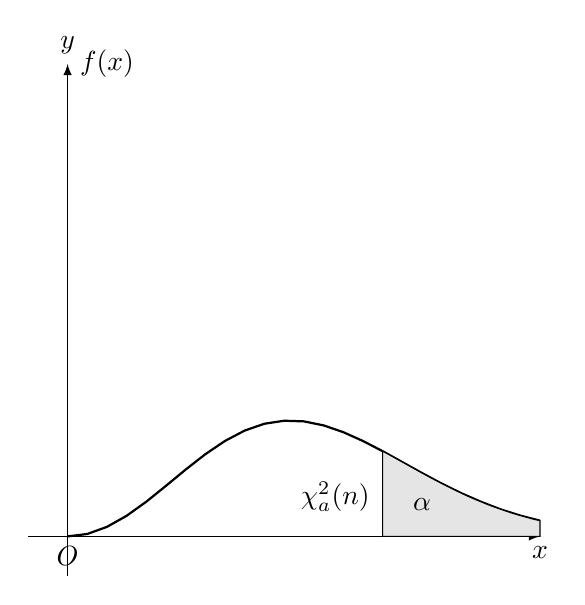
\begin{tikzpicture}[scale=2]
    \draw[-latex](-0.25,0) -- (3,0) node[below]{$x$};
    \draw[-latex](0,-0.25) -- (0,3) node[above]{$y$};
    \filldraw[black] (0,0) node[below]{$O$};
    \draw[black, thick, domain=0:3] plot (\x,{pow(\x,2)*pow(e,-\x*\x/2)});
    \filldraw[black] (1.7,0.25) node{$\chi_a^2(n)$};
    \filldraw [fill=gray!20] (2,0) -- (2,0.5) --  plot [domain=2:3,smooth] (\x,{pow(\x,2)*pow(e,-\x*\x/2)}) -- (3,0) -- (2,0);
    \filldraw[black] (0.25,3) node{$f(x)$};
    \filldraw[black] (2.25,0.2) node{$\alpha$};
\end{tikzpicture}

\paragraph{性质} \leavevmode \medskip 

\begin{itemize}
    \item 若$X_1\sim\chi^2(n_1)$,$X_2\sim\chi^2(n_2)$,$X_1X_2$相互独立,则$X_1+X_2\sim\chi^2(n_1+n_2)$。一般,若$X_i\sim\chi^2(n_i)$($i=1,2,\cdots,m$),$X_1,X_2,\cdots,X_m$相互独立,则$\sum\limits_{i=1}^mX_i\sim\chi^2\left(\sum\limits_{i=1}^mn_i\right)$。
    \item 若$X\sim\chi^2(n)$,则$EX=n$,$DX=2n$。
\end{itemize}

\subsubsection{\texorpdfstring{$t$分布}{}}

\paragraph{概念} \leavevmode \medskip

也称为学生分布。

若随机变量$X\sim N(0,1)$,$Y\sim\chi^2(n)$,$XY$相互独立,则随机变量$t=\dfrac{X}{\sqrt{Y/n}}$服从自由度为$n$的$t$分布,记为$t\sim t(n)$。

当$t\to\infty$时,$t$分布就是正态分布。其是偶函数,所以$Et=0$。

\subsubsection{\texorpdfstring{$F$分布}{}}

若随机变量$X_1,X_2,\cdots,X_n$

\subsection{正态总体下结论}

\section{参数点估计}

\subsection{概念}

\subsection{方法}

\subsubsection{矩估计法}

\subsubsection{最大似然估计}

\subsection{估计量平均标准}

\subsubsection{无偏性}

\subsubsection{有效性}

最小方差性。

\subsubsection{一致性}

相合性。

\section{参数区间估计与假设检验}

\subsection{区间估计}

\subsubsection{概念}

\subsubsection{正态总体均值的置信空间}

\subsection{检设检验}

\subsubsection{思想}

\subsubsection{正态总体下的六大检验与拒绝域}

\subsection{两类错误}

\end{document}
